%% VCL2026 -- Hội thảo Quốc gia lần 4 về Ngôn ngữ học Tính toán
%% Bố cục dựng theo ĐÚNG file "VCL_Conference_Paper_Template for authors.docx"
%% (bản chính thức ban tổ chức phát cho tác giả; thông số đọc trực tiếp từ XML của file đó):
%%   khổ A4 · lề 2,54 cm CẢ BỐN PHÍA · Times New Roman 12
%%   giãn dòng 1,5 ở thân bài (theo thông báo hội thảo; template ghi "đôi" -- xem README)
%%   tóm tắt · trích dẫn khối · bảng · tài liệu tham khảo: giãn ĐƠN
%%   thụt đầu dòng 0,5 inch = 36pt · cách đoạn trước 0pt, sau 6pt
%%   nhan đề đậm 14 canh giữa · tác giả nghiêng canh giữa, nối tên cuối bằng "&"
%%   mục cấp 1: SỐ Ả RẬP "1." đậm CANH GIỮA · cấp 2 "1.1." đậm-nghiêng canh trái
%%   cấp 3 "1.1.1." nghiêng canh trái
%%   bảng kiểu APA: KHÔNG kẻ dọc, chỉ ba đường ngang; nhan đề đặt TRÊN bảng,
%%     "Bảng n" đậm ở dòng riêng rồi tiêu đề nghiêng ở dòng dưới, canh trái
%%   ghi chú bảng đặt dưới, cỡ 9
%%   tài liệu tham khảo: APA 7th, xếp theo bảng chữ cái, THỤT TREO 0,5 inch, sang trang mới
%%   cuối bài: Bionote + thông tin liên hệ theo quy định hội thảo
%% DỰNG: tectonic -X compile main.tex --outdir . --keep-logs   (máy này KHÔNG có xelatex)
\documentclass[12pt,a4paper,onecolumn]{article}

%% ---------------- FORMAT (đổi ở đây nếu CFP đổi) ----------------
\usepackage[a4paper,margin=2.54cm,headheight=15pt,headsep=13pt,footskip=1.15cm]{geometry}
\usepackage{fontspec}
\setmainfont{texgyretermes}[
  Extension = .otf, UprightFont = *-regular, BoldFont = *-bold,
  ItalicFont = *-italic, BoldItalicFont = *-bolditalic ]
\setsansfont{texgyreheros}[
  Extension = .otf, UprightFont = *-regular, BoldFont = *-bold,
  ItalicFont = *-italic, BoldItalicFont = *-bolditalic ]
\setmonofont{texgyrecursor}[
  Extension = .otf, UprightFont = *-regular, BoldFont = *-bold,
  ItalicFont = *-italic, BoldItalicFont = *-bolditalic, Scale = MatchLowercase ]
\usepackage{setspace}
\setstretch{1.5}
\setlength{\parindent}{36pt}
\setlength{\parskip}{6pt plus 1pt minus 1pt}
\emergencystretch=1.2em  % tránh tràn lề ở các chuỗi mã dài

%% -- template KHÔNG có tiêu đề chạy trang; chỉ giữ số trang ----------
\usepackage{fancyhdr}
\pagestyle{fancy}
\fancyhf{}
\fancyfoot[C]{\fontsize{12}{14}\selectfont\thepage}
\renewcommand{\headrulewidth}{0pt}
\renewcommand{\footrulewidth}{0pt}
%% ---------------------------------------------------------------

\usepackage{polyglossia}
\setmainlanguage{vietnamese}
\setotherlanguage{english}
\usepackage{amsmath}
\usepackage{graphicx}
\usepackage{tikz}
\usetikzlibrary{positioning,arrows.meta,fit,calc}
%% ba màu dùng trong Hình 2, khớp đúng giá trị RGB của lớp vẽ trong tệp ảnh
\definecolor{hinhxanhla}{RGB}{34,200,120}
\definecolor{hinhcam}{RGB}{214,140,30}
\definecolor{hinhxanhduong}{RGB}{40,140,215}
\newcommand{\ôvuông}[2]{\tikz[baseline=-0.45ex]{\draw[#1,line width=0.9pt,#2] (0,0) rectangle (0.34,0.18);}}
\usepackage{array}
\usepackage{booktabs}     % bảng kiểu APA: chỉ đường ngang
\usepackage{enumitem}
\usepackage{indentfirst}
\usepackage{url}
\usepackage[hidelinks]{hyperref}
%% DOI: chi ngat dong sau dau gach cheo, khong ngat giua "doi.org"
\def\UrlBreaks{\do\/}
\setlength{\Urlmuskip}{0mu plus 2mu}
\urlstyle{same}

%% -- đánh số mục theo template: cấp 1 số Ả Rập, đậm, CANH GIỮA ---
\renewcommand{\thesection}{\arabic{section}}
\renewcommand{\thesubsection}{\arabic{section}.\arabic{subsection}}
\usepackage{titlesec}
\titleformat{\section}[block]
  {\normalsize\bfseries\centering}{\thesection.}{0.5em}{}
\titlespacing{\section}{0pt}{12pt plus 2pt}{0pt}
\titleformat{\subsection}[block]
  {\normalsize\bfseries\itshape}{\thesubsection.}{0.5em}{}
\titlespacing{\subsection}{0pt}{9pt plus 2pt}{0pt}
\titleformat{\subsubsection}[block]
  {\normalsize\itshape}{\thesubsubsection.}{0.5em}{}
\titlespacing{\subsubsection}{0pt}{9pt plus 2pt}{0pt}

%% -- nhan đề bảng/hình kiểu APA: nhãn ĐẬM dòng riêng, tiêu đề NGHIÊNG
%%    dòng dưới, canh trái, ĐẶT TRÊN bảng/hình -----------------------
\usepackage{caption}
\DeclareCaptionFormat{apa}{\setstretch{1.0}\raggedright\textbf{#1}\par#3\par}
%% template: nhan đề HÌNH canh giữa (style RALs-FigureCaption), khác nhan đề BẢNG canh trái
\DeclareCaptionFormat{apafig}{\setstretch{1.0}\centering\textbf{#1}\par#3\par}
\captionsetup{format=apa, labelsep=none, singlelinecheck=false,
              textfont=it, skip=4pt, belowskip=4pt}
\captionsetup[figure]{format=apafig}
\renewcommand{\tablename}{Bảng}
\renewcommand{\figurename}{Hình}
%% ghi chú dưới bảng: template style RALs-TableNote = 9 pt, giãn đơn
\newcommand{\tablenote}[1]{\par\vspace{2pt}{\setstretch{1.0}\fontsize{9}{11}\selectfont\raggedright\noindent #1\par}}
%% nội dung bảng: template ghi rõ 10 pt (style RALs-APA-Table, sz=20 half-point)
\newcommand{\bangchu}{\fontsize{10}{12}\selectfont}

%% -- tài liệu tham khảo APA 7th: không đánh số, thụt treo 0,5 inch -
\newenvironment{apareferences}{%
  \newpage
  \section*{TÀI LIỆU THAM KHẢO}%
  \setstretch{1.0}%
  \sloppy%
  \setlength{\parindent}{0pt}%
  \setlength{\parskip}{6pt plus 1pt}%
  \begin{list}{}{%
    \setlength{\leftmargin}{36pt}%
    \setlength{\itemindent}{-36pt}%
    \setlength{\listparindent}{0pt}%
    \setlength{\labelwidth}{0pt}%
    \setlength{\labelsep}{0pt}%
    \setlength{\itemsep}{6pt}%
    \setlength{\parsep}{0pt}%
    \setlength{\topsep}{0pt}}%
}{\end{list}}
\newcommand{\apaitem}{\item[]}

\newcommand{\code}[1]{{\small\texttt{#1}}}
\begin{document}

%% ================= KHỐI NHAN ĐỀ =================
%% Template: nhan đề đậm 14 canh giữa · tác giả NGHIÊNG canh giữa, nối "&"
%% Đơn vị công tác KHÔNG đặt ở cước chú -- template đưa xuống mục Bionote cuối bài.
\begin{center}
{\setstretch{1.1}\fontsize{14}{17}\selectfont\bfseries
SINH BIỂU THỨC QUY CHIẾU CHO PHẦN TỬ GIAO DIỆN:\\
XÂY DỰNG NGỮ LIỆU TỰ ĐỘNG KHI PHẦN TỬ\\
KHÔNG CÓ TÊN ĐỂ GỌI\par}
\vspace{8pt}
{\setstretch{1.0}\itshape Lê Đoàn Phương Uyên \& Nguyễn Hồng Bửu Long\par}
\end{center}
\vspace{6pt}

%% -- Tóm tắt: tiêu đề đậm không thụt, nội dung giãn ĐƠN, không thụt đầu dòng --
{\noindent\bfseries Tóm tắt\par}
{\setstretch{1.0}\noindent
Sinh hướng dẫn thao tác từ ảnh màn hình và mục tiêu người dùng là bài toán sinh biểu
thức quy chiếu, nhưng $22{,}0\%$ phần tử cần chạm lại không có tên. Mỗi bước chạm của
AndroidControl có một dòng mô tả gồm vai trò, tên, toạ độ và một dấu hiệu tách phần tử
ấy khỏi những phần tử giống nó; cả $41.099$ dòng do luật sinh ra, không nhãn nào do
người viết. $75{,}3\%$ dấu hiệu thuộc loại tự nó đủ tách, nhưng riêng ở nhóm chỉ mang
một ký hiệu thì tỉ lệ ấy còn $37{,}5\%$. Quy trình không đọc câu chỉ dẫn do người viết,
nên đây là một phép so độc lập. Ở đó, $53{,}5\%$ ô tên trùng nguyên văn với câu ấy, gấp
bảy lần đối chứng ghép sang bước kế cùng chuỗi. Bộ phép kiểm bắt bốn lỗi vốn không hề lộ ra.
\par}

%% -- Từ khoá: nhãn đậm-nghiêng, thụt 0,5 inch, chữ thường --
{\setstretch{1.0}\hspace*{36pt}\textit{Từ khoá}: sinh biểu thức quy chiếu, dấu hiệu phân
biệt, giao diện đồ hoạ, xây dựng ngữ liệu tự động, kiểm chất lượng dữ liệu,
AndroidControl\par}
\vspace{6pt}

\section{Đặt vấn đề}
\label{sec:datvande}

Một tác tử điều khiển giao diện (\emph{GUI agent}) thường nhận câu chỉ dẫn rồi trả về toạ
độ thao tác tương ứng, còn chúng tôi giải quyết bài toán ngược lại. Hệ thống nhận vào ảnh chụp
màn hình cùng mục tiêu của người dùng, và từ đó phải viết ra \emph{một câu} đủ để người đọc
câu ấy biết phải chạm vào đâu, chẳng hạn ``chạm vào biểu tượng bút chì ở góc trên bên phải
của ghi chú''. Các hệ thống theo hướng này đã bắt đầu xuất hiện trong ứng dụng trợ
năng và hỗ trợ người dùng lớn tuổi (Fang và cộng sự, 2026). Về mặt ngôn ngữ, đây là bài
toán \emph{sinh biểu thức quy chiếu} (referring expression generation), trong đó câu sinh ra
phải đủ để người nghe nhận ra đúng một đối tượng, không lẫn với những đối tượng khác
cùng có mặt. Khung khái niệm
ấy đã có sẵn từ dòng nghiên cứu tóm tắt ở Mục~\ref{sec:lienquan}; đóng góp của bài nằm ở
việc chuyển nó sang một miền mà phương tiện gọi tên gần như không có sẵn.

Các số liệu sau cho thấy đặc thù đó, tất cả đều do chúng tôi đo trên chính ngữ liệu dùng
trong bài. Mỗi màn hình Android đi kèm một \emph{cây trợ năng} (\emph{accessibility tree}), nghĩa là
bản kết xuất từ view hierarchy của ứng dụng, liệt kê các phần tử đang hiển thị cùng nhãn
văn bản của từng phần tử. Chúng tôi đo trên $120$ màn lấy ngẫu nhiên từ kho $99.131$ màn,
và chỉ $12{,}6\%$ phần tử mang được một nhãn văn bản nào đó, trong khi $22$ trên $120$ màn
không có lấy một phần tử nào mang tên. Kết quả
này khớp với các khảo sát cho thấy phần lớn ứng dụng Android xuất xưởng với nhãn trợ năng
không đầy đủ (Chen và cộng sự, 2020). Trên $41.099$ nhãn dựng được, $22{,}0\%$ phần tử cần chạm không có tên nào để gọi, và
$7{,}6\%$ trùng tên với ít nhất một phần tử khác trên cùng màn hình. Một phần tử đã không có tên thì cũng không thể trùng tên với phần tử khác,
nên hai nhóm không chồng lên nhau và cộng thẳng lại được, cho
$12.162/41.099 = 29{,}6\%$. Ở
gần một phần ba số ca, người viết câu buộc phải quy chiếu bằng \emph{vị trí} hoặc bằng
\emph{quan hệ với chữ lân cận}.

Điều đó tác động trực tiếp sang phía mô hình. Khi không có tên để gọi, câu sinh ra dễ
viện
tới một tên gọi hợp lý về mặt ngôn ngữ nhưng không tồn tại trên màn hình, còn người dùng
thì không có căn cứ nào để nhận ra mình đang bị chỉ sai. Nền dữ liệu vì vậy phải ghi được
cả những ca \emph{không} gọi tên được và nêu rõ khi đó lấy gì thay thế, thay vì loại chúng
khỏi tập giám sát để các chỉ số tổng hợp cao hơn. Hậu quả của việc chỉ sai cũng không như nhau với mọi người dùng. Người đọc màn hình bằng
tai qua trình đọc trợ năng, hay người lớn tuổi lần đầu dùng một ứng dụng, vừa là nhóm khó
tự phát hiện mình bị chỉ nhầm nhất, vừa là nhóm phụ thuộc nhiều nhất vào số ít phần tử có
nhãn trợ năng, đúng bằng $12{,}6\%$ nói trên, vì trình đọc màn hình chỉ đọc được những phần
tử ấy.

Huấn luyện mô hình cho tác vụ này đòi hỏi dữ liệu giám sát, trong khi chưa có bộ dữ liệu
công khai nào được dựng sẵn cho mục đích đó. Bài báo trình bày cách chúng tôi dựng dữ liệu giám sát từ AndroidControl (W. Li và cộng sự, 2024) hoàn toàn tự động, cùng những
phép kiểm đã bắt được lỗi trong quá trình dựng. Cụm từ \emph{tự động hoàn toàn} cần được phân định ngay, bởi người vẫn có tham gia vào quy
trình, nhưng chỉ ở khâu \emph{kiểm} chứ không ở khâu dán nhãn.
Không nhãn nào trong $41.099$ nhãn được người viết, sửa hay chọn; các lượt đọc thủ công chỉ dùng để phát hiện luật sai, và thứ được sửa mỗi lần như vậy là bản thân bộ luật, sau đó
toàn bộ nhãn được dựng lại từ đầu. Phần đo lường chất lượng câu sinh ra và các kết quả
huấn luyện nằm ở một bài đồng hành của cùng nhóm tác giả, hiện đang bình duyệt (Lê \&
Nguyễn, 2026).

Bài báo có ba đóng góp. Đóng góp thứ nhất là một quy trình tự động dựng nhãn mô tả có cấu
trúc cho $41.099$ bước, kèm hai bộ lọc được thêm vào sau khi đo thấy nhãn bị nhiễu. Đóng góp thứ hai
là một bộ phép kiểm dựng dữ liệu dùng lại được cho các quy trình dán nhãn tự động khác,
gồm một đối chứng lệch chủ ý, là phép ghép cố ý làm sai để lấy mức tham chiếu, chín bất
biến cấu trúc, phép kiểm rò rỉ chạy trên toàn bộ dữ liệu, và một phép đối chiếu ô tên của
nhãn với chính câu do người viết. Đóng góp thứ ba là một phân tích chiến lược quy chiếu
trên $41.099$ nhãn cùng $41.084$ câu do người viết, cho thấy trong miền giao diện, cả người viết lẫn quy trình tự động
đều chuyển từ lối gọi tên sang lối định vị theo quan hệ, trong khi nguồn quan hệ hiện có
lại phủ kém nhất đúng ở nhóm phần tử cần nó nhất. Bài còn kèm theo bốn ca lỗi thật, mỗi ca cho biết phép kiểm nào bắt được loại lỗi nào.

\section{Công trình liên quan}
\label{sec:lienquan}

\subsection{Sinh biểu thức quy chiếu}
Dale và Reiter (1995) đặt bài toán ở dạng chọn thuộc tính, với yêu cầu rằng mô tả phải đủ
để người nghe tách được đối tượng đích, đồng thời không thừa tới mức kéo theo hàm ý sai. Khi thuộc tính
riêng không đủ tách, Dale và Haddock (1991) chuyển sang mô tả \emph{quan hệ}, nghĩa là định vị đối tượng qua một đối tượng khác đã xác định được; Krahmer và van Deemter (2012) tổng kết
hai thập niên của dòng này. Trên ảnh, Mao và cộng sự (2016) chuyển tiêu chí phân biệt
thành mục tiêu huấn luyện, còn Luo và Shakhnarovich (2017) cùng Yu và cộng sự (2017) đưa
một mô hình ``người nghe'' vào vòng huấn luyện để ép tính phân biệt. Toàn bộ dòng này đều xét ảnh tự nhiên, nơi đối tượng hầu như luôn có một danh từ để gọi, nên quan hệ là
phương án \emph{bổ sung} khi danh từ chưa đủ tách. Miền giao diện đảo ngược quan hệ ấy, bởi ở $22{,}0\%$ phần tử cần chạm thì danh từ để gọi
không hề tồn tại, nên quan hệ trở thành phương tiện quy chiếu duy nhất còn lại. Chúng tôi
giữ nguyên khung khái niệm đó và đo dấu vết mà sự đảo chiều ấy để lại trong phân bố nhãn.

\subsection{Mô tả phần tử giao diện}
Widget Captioning (Y. Li và cộng sự, 2020b) là công trình gần nhất trong miền này, vì nó cũng sinh mô tả ngôn ngữ cho phần tử giao
diện di động và cũng nêu vấn đề các widget trông giống hệt nhau, nhưng huấn luyện bằng
cross-entropy thuần. Giữa công trình đó và bài này có ba điểm phân định. Về nguồn nhãn, nhãn của họ
do người viết qua thu thập cộng đồng, còn nhãn của chúng tôi dựng bằng luật, nên rẻ hơn nhiều bậc và phủ quy mô lớn hơn, nhưng nghèo hơn về chất lượng ngôn ngữ mà chúng tôi lại
không có đánh giá bằng người để định lượng khoảng cách đó. Về đơn vị chú thích, họ mô tả
\emph{một widget} tách khỏi ngữ cảnh, còn ở đây phần tử cần chạm luôn nằm trong một màn hình
cụ thể với các phần tử cạnh tranh cụ thể, nên tính phân biệt là thuộc tính của cặp (phần
tử, màn hình). Về vai trò của nhãn, nhãn của chúng tôi là phần mô hình phải sinh ra
\emph{trước} câu chỉ dẫn, chứ không phải sản phẩm cuối. Ở
mức \emph{màn hình}, Screen2Words (Wang và cộng sự, 2021) cho thấy dòng mô tả giao diện
bằng ngôn ngữ đã có sẵn cả hai mức, và mức phần tử là mức mà tính phân biệt trở thành ràng
buộc bắt buộc. Chen và cộng sự (2020) dự đoán nhãn trợ năng còn thiếu cho phần tử Android, cũng là hiện tượng ``phần tử không có tên'' mà chúng tôi đo lại được trên một ngữ liệu
khác; hướng của họ là \emph{bù} nhãn thiếu bằng mô hình, hướng của chúng tôi là chấp nhận
nhãn thiếu và chuyển nhiệm vụ quy chiếu sang quan hệ với chữ lân cận.

\subsection{Ngữ liệu điều khiển giao diện}
AndroidControl (W. Li và cộng sự, 2024) cung cấp $15.283$ chuỗi thao tác do người thật ghi
lại, mỗi bước có một câu chỉ dẫn do người viết và một toạ độ chạm. Trong bài gốc, câu chỉ
dẫn theo bước là \emph{đầu vào} để dự đoán thao tác; ở đây nó chính là \emph{đầu ra mong
đợi} của mô hình. Chiều ``câu chỉ dẫn làm đầu vào'' là chiều quen thuộc của cả dòng, từ
Seq2act (Y. Li và cộng sự, 2020a) tới AndroidInTheWild (Rawles và cộng sự, 2023); việc đưa
danh sách phần tử màn hình vào \emph{đầu vào} cũng đã phổ biến (Deng và cộng sự, 2023;
W. Li và cộng sự, 2024; Y. Li và cộng sự, 2020b). Điểm khác ở đây nằm ở phía đối diện, vì mô tả phần tử là thứ mô hình phải \emph{sinh ra}
chứ không phải một trường dữ liệu được cấp sẵn, nên nó phải đủ để một bên thứ ba trỏ
đúng.

\section{Nguồn dữ liệu và phép ghép đa nguồn}
\label{sec:nguon}

Mỗi bước cần đủ ba thành phần: câu chỉ dẫn do người viết, ảnh màn hình, và cây trợ
năng. Không bản phát hành công khai nào của AndroidControl mang đủ cả ba
(Bảng~\ref{tab:nguon}), nên chúng tôi phải ghép hai bản lại với nhau.

\begin{table}[t]
\centering\setstretch{1.0}\bangchu

\renewcommand{\arraystretch}{1.25}
\caption{Hai bản phát hành trên Hugging Face và phần thiếu của mỗi bản.}
\label{tab:nguon}
\begin{tabular}{p{5.3cm}p{4.3cm}p{4.6cm}}
\toprule
\textbf{Kho} & \textbf{Có} & \textbf{Thiếu} \\
\midrule
\code{HarrytheOrange/}\newline\code{\ \ parsed\_AndroidControl}
 & câu chỉ dẫn đủ $15.283$ chuỗi; cây trợ năng $99.131$ màn & không có ảnh \\
\code{ckg/AndroidControl}\newline\code{\ \ ParsedWithImages-20k}
 & ảnh màn hình & đã chuyển sang định dạng tác tử nên mất câu chỉ dẫn theo bước \\
\bottomrule
\end{tabular}

\end{table}

Chúng tôi ghép hai kho theo khoá \code{(episode\_id, step\_id)}. Bản phát hành còn một tính
chất phải nêu ra, vì nó ảnh hưởng tới cách đọc mọi kết quả về sau, đó là chuỗi mục tiêu, nghĩa là câu mô tả mục tiêu chung của cả tác vụ, bị cắt ngay từ nguồn, chẳng hạn \code{...look for Calvin Kle}. Đo trên $1.424$ mục tiêu khác nhau của
tập kiểm, $99{,}4\%$ không kết thúc bằng một dấu câu và ít nhất $71{,}3\%$ kết thúc giữa
chừng một từ; chúng tôi nói ``ít nhất'' vì luật đếm chỉ nhận những từ cuối không hề xuất
hiện ở vị trí nào khác trong ngữ liệu, nên nó bỏ sót mọi ca mà phần bị cắt tình cờ trùng
một từ có thật. Mọi nhánh dữ liệu dựng từ bộ nhãn này (Phụ lục~A) đều đọc cùng chuỗi bị cắt đó, nên hiện
tượng cắt này không giải thích được chênh lệch \emph{giữa} các nhánh, nhưng nó có thật và không sửa được từ phía chúng
tôi.

\emph{Phép kiểm ghép.} Ghép lệch một bước là loại lỗi nguy hiểm nhất trong quy trình này, vì số dòng vẫn đủ, huấn
luyện vẫn hội tụ và mọi khâu phía sau vẫn chạy bình thường, trong khi mô hình đang học ảnh
của bước $A$ với câu của bước $B$ mà không khâu nào báo lỗi.

Chúng tôi thiết kế phép kiểm sao cho lỗi đó buộc phải lộ ra, bằng cách chạy OCR tại điểm
chạm đáp án rồi xem chuỗi chữ đọc được có xuất hiện trong câu chỉ dẫn hay không. Nếu ghép đúng, tỉ lệ khớp phải cao
hơn hẳn so với một \emph{đối chứng lệch chủ ý một bước}, nghĩa là phép ghép cố ý làm sai bằng cách lấy ảnh và điểm chạm của bước này đem so với câu chỉ dẫn của bước liền sau. Trên $400$
bước lấy mẫu, ghép đúng cho $48{,}3\%$ ($193/400$; khoảng tin cậy Wilson $95\%$:
$[43{,}4;\ 53{,}1]$); đối chứng chạy trên $311$ bước, vì bước cuối mỗi chuỗi không có bước
kế để ghép lệch sang, và cho $19{,}6\%$ ($61/311$; $[15{,}6;\ 24{,}4]$). Tỉ số giữa hai bên là $2{,}5$ lần, và hai khoảng tin cậy cách nhau $19$ điểm phần trăm.

Về mặt phương pháp, giá trị của phép kiểm không nằm ở con số $48\%$, vì tự nó không mang
thông tin, bởi OCR có lỗi còn người viết câu cũng không nhất thiết nhắc lại chữ in trên
nút. Con số ấy chỉ diễn giải được khi đặt cạnh mức $20\%$ của đối chứng, và thứ đọc được là
khoảng cách giữa hai bên. Phép kiểm này cũng có phạm vi hẹp, vì nó chỉ bắt \emph{lỗi ghép
có hệ thống} trên toàn ngữ liệu chứ không xác nhận từng dòng, nên một lỗi lệch ngẫu nhiên
chạm tới vài phần trăm số dòng vẫn lọt qua. Chúng tôi chọn nó vì nó rẻ, chạy lại được sau mỗi lần dựng, và vì
loại lỗi nó nhắm là loại duy nhất phá hỏng \emph{toàn bộ} tập giám sát trong khi mọi khâu
vẫn chạy tới cuối.

\section{Trích chữ trên màn hình}
\label{sec:ocr}

Cây trợ năng lẽ ra là nguồn tên phần tử tự nhiên, nhưng trên mẫu $120$ màn đã nêu ở Mục~\ref{sec:datvande}, chỉ $12{,}6\%$ phần tử mang bất
kỳ tên nào, khớp với ghi nhận của Chen và cộng sự (2020), và
bản kết xuất đang có còn chứa cả \code{content\_\allowbreak description}, là trường mô tả dành cho trình đọc màn hình, thường do lập trình viên đặt và không trùng với chữ thật
hiển thị trên màn. Một màn có trung vị $86$ phần tử, nhưng phần lớn số đó không mang nhãn
văn bản nào.

Vì vậy toàn bộ ảnh màn hình được đưa qua nhận dạng ký tự quang học (RapidOCR, ONNX, chỉ
chạy trên CPU), kết quả vừa làm đặc trưng đầu vào vừa làm nguồn tên phần tử. Khâu này thu được $64.567$
bản ghi cho tập dạy và $6.958$ cho tập kiểm, không thiếu bản nào. Chúng tôi chạy lại nó
trên hai máy khác nhau, cách nhau năm ngày, và kết quả trùng nhau; mật độ chuỗi nhận dạng được cũng đồng đều giữa hai tập
($24{,}2$ chuỗi mỗi màn ở tập kiểm so với $23{,}6$ ở tập dạy).

Vì AndroidControl không có nhãn chuẩn cho chữ trên màn, chúng tôi \emph{không} tuyên bố độ
chính xác của OCR. Hai dạng sai sót quan sát được là biểu tượng bị đọc thành ký tự, và
khoảng trắng giữa hai từ bị mất, cho ra những chuỗi dính liền như \code{Turnon}. Dạng thứ
nhất nguy hiểm hơn vì nó sinh ra một chuỗi trông như tên thật, và khi không có nhãn chuẩn
thì tần suất của nó không đo trực tiếp được (Mục~\ref{sec:hanche}). Dạng thứ hai chỉ đẩy
phần tử xuống nhóm ``không có tên'', nên nhiệm vụ quy chiếu chuyển sang ô thứ tư của nhãn, là ô dấu hiệu phân biệt được mô tả
ở Mục~\ref{sec:nhan}, và bản thân nhãn vẫn không chứa thông tin sai về màn hình. Đối với một nguồn giám sát,
lỗi \emph{bỏ sót} rẻ hơn hẳn lỗi \emph{gán sai}, vì nhãn để trống chỉ làm mô hình mất một
mẫu học, còn nhãn mang tên sai thì dạy mô hình gọi phần tử bằng một chuỗi không tồn tại
trên màn hình. Hai bộ lọc ở Mục~\ref{sec:cong} là chỗ nguyên tắc đó được thi hành, vì khi tên không kiểm
chứng được thì chúng để ô tên trống, thay vì điền vào đó một chuỗi phỏng đoán.

\section{Nhãn mô tả bốn ô}
\label{sec:nhan}

Cách dựng nhãn dưới đây dùng tới \emph{hộp bao} (\emph{bounding box}), là hình chữ nhật mà
cây trợ năng ghi cho mỗi phần tử để cho biết phần tử ấy chiếm vùng nào trên màn.

Chuỗi mà mô hình phải học để sinh ra, gọi là \emph{đầu ra mong đợi}, mở đầu bằng một dòng \emph{nhãn mô tả} (\emph{descriptor}) có cấu trúc, mô tả phần tử cần
chạm. Nhãn này chỉ
dựng cho \emph{bước chạm}, nghĩa là bước mà thao tác đúng là một cú chạm lên màn hình; các loại
bước khác không mang nhãn mô tả. Dòng này dựng hoàn toàn bằng luật, theo bốn bước, mỗi bước điền một \emph{ô}, là một trường thông tin trong dòng ấy. Bước chuẩn bị là xác định phần tử cần chạm, bằng cách lấy toạ độ ghi trong đáp án rồi chọn
hộp bao nhỏ nhất có chứa điểm đó. Việc chọn hộp \emph{nhỏ nhất} là cần thiết vì cây trợ năng lồng nhiều tầng, nên một điểm chạm
thường nằm bên trong hàng chục hộp cùng lúc, từ khung bao cả màn hình cho tới nút thật sự
bị bấm. Hình~\ref{fig:quytrinh} tóm tắt cả đường đi này, kèm chỗ mà mỗi bộ lọc can thiệp và
tỉ lệ dữ liệu mà nó động tới.

\begin{figure}[t]
\centering\setstretch{1.0}
\caption{Đường đi từ một bước thao tác tới dòng nhãn bốn ô, cùng chỗ mà mỗi bộ lọc can thiệp.}
\label{fig:quytrinh}
\begin{tikzpicture}[
  font=\footnotesize,
  node distance=4.5mm,
  ô/.style={draw,rounded corners=2pt,align=left,inner sep=5pt,text width=7.4cm},
  ghi/.style={align=left,inner sep=3pt,text width=5.4cm,font=\scriptsize\itshape,gray!55!black},
  mũi/.style={-{Latex[length=2.2mm]},gray!60},
  đứt/.style={dashed,gray!55,shorten >=1pt}
]
\node[ô,fill=gray!8] (a) {\textbf{Đầu vào của một bước}\\ ảnh màn hình · cây trợ năng · điểm chạm ghi trong đáp án};
\node[ô,below=of a] (b) {\textbf{Xác định phần tử cần chạm}\\ chọn hộp bao nhỏ nhất có chứa điểm chạm};
\node[ô,below=of b] (c) {\textbf{Ô vai trò và ô toạ độ}\\ tên lớp Android quy về một từ; điểm chạm quy về thang $0$ tới $1.000$};
\node[ô,below=of c] (d) {\textbf{Ô tên}\\ lấy chuỗi ở cây trợ năng trước, chuỗi OCR nằm trong hộp bao sau};
\node[ô,below=of d] (e) {\textbf{Ô dấu hiệu phân biệt}\\ chuỗi OCR gần nhất nằm ngoài hộp bao, cách tâm không quá $350$ px, kèm hướng};
\node[ô,below=of e,fill=gray!8] (f) {\textbf{Dòng nhãn}\\ \code{<desc>icon | (no name) | <point>111,903</point> | just above the text “Gmail”</desc>}};

\foreach \x/\y in {a/b,b/c,c/d,d/e,e/f} \draw[mũi] (\x) -- (\y);

\node[ghi,right=6mm of b.east,anchor=west] (nb) {cây trợ năng lồng nhiều tầng nên một điểm chạm nằm trong hàng chục hộp cùng lúc};
\node[ghi,right=6mm of d.east,anchor=west] (nd) {bộ lọc nhãn trợ năng loại $14{,}7\%$ chuỗi ở lát thử; bộ lọc hình học bỏ hộp phủ quá $25\%$ màn; không nguồn nào cho được chuỗi dùng được thì ô tên là \code{(no name)}, gặp ở $22{,}0\%$ bước};
\node[ghi,right=6mm of e.east,anchor=west] (ne) {không có chuỗi nào đủ gần thì luật lùi về mệnh đề duy nhất, trùng tên hoặc đếm; $75{,}3\%$ dấu hiệu tự nó đủ tách};

\draw[đứt] (b.east) -- (nb.west);
\draw[đứt] (d.east) -- (nd.west);
\draw[đứt] (e.east) -- (ne.west);
\end{tikzpicture}
\end{figure}

\begin{itemize}[leftmargin=1.8em,itemsep=0.25em]
\item \textbf{Ô vai trò} lấy thẳng từ cây trợ năng, sau khi quy tên lớp Android về một từ
người đọc hiểu được, chẳng hạn \code{tappable text}; ô này phân biệt nút, ô nhập và mục
danh sách.
\item \textbf{Ô tên} là chữ hiển thị, chẳng hạn \code{Search here}. Chương trình lấy chuỗi từ cây trợ năng nếu
chuỗi ở đó qua được bộ lọc mô tả ở Mục~\ref{sec:cong}; nếu chuỗi bị loại thì nó chuyển sang
lấy chuỗi OCR nằm bên trong hộp bao; còn nếu cả hai nguồn đều không cho được chuỗi nào
dùng được thì ô tên để trống.
\item \textbf{Ô toạ độ} giữ chính điểm chạm, quy về thang từ $0$ tới $1.000$ theo chiều
rộng và chiều cao, để không phụ thuộc độ phân giải của từng ảnh. Đây là ô duy nhất chép thẳng từ đáp án, nên nó không thể sai và cũng không tốn công dựng.
\item \textbf{Ô dấu hiệu phân biệt} giữ một mệnh đề do luật tính ra, chẳng hạn \code{just
above the text “Coffee”}. Ô này tách phần tử cần chạm khỏi những phần tử giống nó, nhắm thẳng vào ca $7{,}6\%$ trùng
tên và $22{,}0\%$ không tên; luật sinh ra mệnh đề này được mô tả ở
Mục~\ref{sec:lamlai}.
\end{itemize}

Một nhãn hoàn chỉnh trông như sau:

\begin{center}\small\ttfamily
<desc>tappable text | Search here | <point>440,91</point> | just above the text
``Coffee''</desc>
\end{center}

Nhãn vừa nêu thuộc ca phần tử cần chạm có tên, còn Hình~\ref{fig:moneo} vẽ lại một bước
thật thuộc ca khó hơn, khi phần tử cần chạm không có tên nào. Ở ca đó, ba ô đầu chỉ định danh được phần tử, còn toàn bộ việc quy chiếu phải
dựa vào ô thứ tư, ở đây là một \emph{mỏ neo chữ}, nghĩa là chuỗi chữ gần nhất nằm bên cạnh và
được dùng làm mốc để chỉ đường.

\begin{figure}[t]
\centering
\caption{Mỏ neo chữ trên một màn hình thật: bốn biểu tượng cùng vai trò, không biểu tượng
nào có tên.}
\label{fig:moneo}
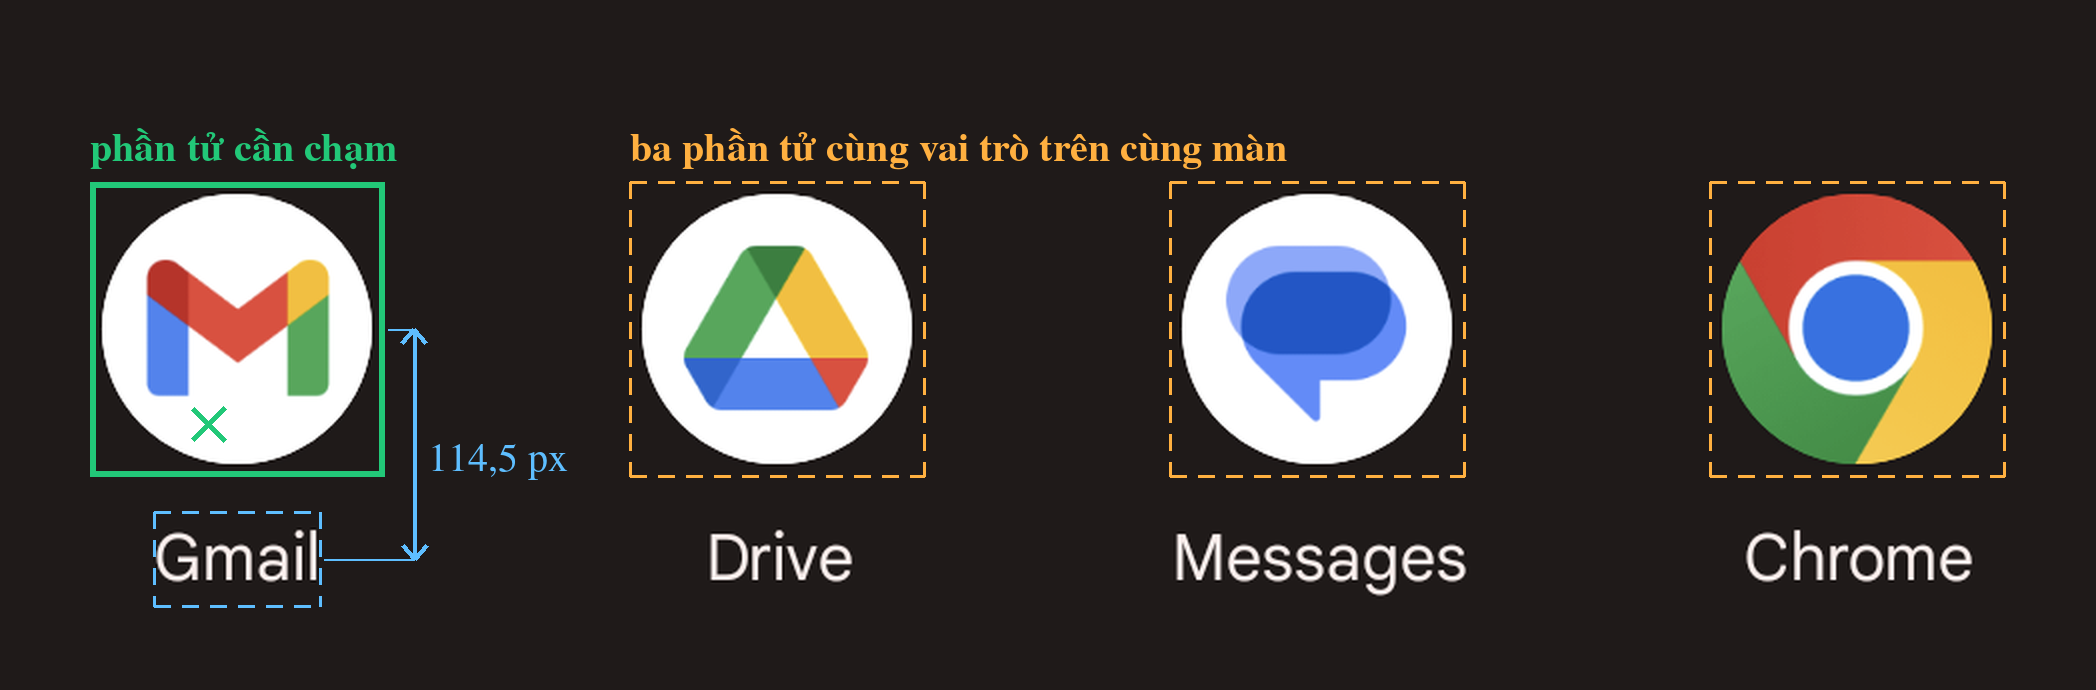
\includegraphics[width=\linewidth]{hinh/fig_moneo.png}

\vspace{5pt}
{\setstretch{1.0}\footnotesize\centering
\code{<desc>icon | (no name) | <point>111,903</point> | just above the text “Gmail”</desc>}\par}

\vspace{5pt}
{\setstretch{1.0}\footnotesize\raggedright\noindent
\textit{Ghi chú.} Ảnh chụp màn hình thật của một bước trong tập kiểm, có phủ thêm lớp vẽ.
Hộp bao, điểm chạm và vị trí chuỗi chữ đều lấy từ cây trợ năng và tệp OCR của chính bước
ấy, nên các khoảng cách trên hình là khoảng cách thật. Khung liền \ôvuông{hinhxanhla}{} là
phần tử cần chạm, còn ba khung nét đứt \ôvuông{hinhcam}{dashed} là ba biểu tượng cùng vai
trò, và không biểu tượng nào trong bốn cái mang tên trong cây trợ năng. Khung nét đứt
\ôvuông{hinhxanhduong}{dashed} là chuỗi OCR gần nhất nằm ngoài hộp bao, cách tâm $114{,}5$
px, nên luật lấy nó làm mỏ neo và sinh ra dòng nhãn ở trên. Câu do người viết cho cùng bước
là \emph{Click on the gmail option}, cũng quy chiếu qua chữ \emph{Gmail}.\par}
\end{figure}

Ô thứ tư là ô mang nội dung ngôn ngữ học của nhãn, vì ba ô đầu chỉ để định danh,
còn ô này mới là chỗ duy nhất nói được rằng trong số những phần tử trông giống nhau trên
màn thì phần tử nào là phần tử cần chạm. Đây chính là thuộc tính phân biệt theo cách gọi
của lý thuyết biểu thức quy chiếu.

\begin{table}[t]
\centering\setstretch{1.0}\bangchu

\renewcommand{\arraystretch}{1.3}
\caption{Bốn nhãn thật lấy nguyên văn từ tập dạy, kèm câu do người viết cho cùng bước.}
\label{tab:vidu}
\begin{tabular}{p{8.4cm}p{5.6cm}}
\toprule
\textbf{Nhãn tự động} & \textbf{Câu do người viết} \\
\midrule
\code{tappable text | Search here | <point>440,91</point> | just above the text
“Coffee”} & \emph{Click on the search bar} \\
\code{icon | (no name) | <point>256,524</point> | just above the text “Leaf”}
 & \emph{Choose the leaf option} \\
\code{icon | Q | <point>920,899</point> | shares a name with 1 other elements on screen}
 & \emph{click on the search icon} \\
\code{icon | (no name) | <point>920,904</point> | many elements of the same kind on
screen} & \emph{Click on the Right arrow key} \\
\bottomrule
\end{tabular}
\tablenote{\textit{Ghi chú.} Ở hai ca đầu, mệnh đề ở ô thứ tư đủ để chỉ ra phần tử nào là phần tử cần chạm; ở hai ca sau, mệnh đề chỉ cho biết trên màn có phần tử giống nó.}

\end{table}

Bảng~\ref{tab:vidu} cho thấy khoảng cách giữa nhãn tự động và câu người viết ở mức từng
ca cụ thể, thứ mà các con số tổng hợp không nêu được. Ở ca thứ hai, phần tử không có tên, nhưng mỏ neo chữ ``ngay trên chữ
\emph{Leaf}'' đã đủ để quy chiếu, và người viết cũng chọn đúng chiến lược ấy khi gọi nó là
\emph{leaf option}. Ở hai ca cuối thì ngược lại, khi nhãn chỉ nói được rằng \emph{có} mơ hồ, còn người viết
gọi thẳng \emph{search icon} và \emph{Right arrow key}. Sở dĩ có
khoảng cách đó là vì người viết câu nhìn thấy \emph{hình dạng} của biểu tượng rồi đặt tên
cho nó, còn quy trình của chúng tôi chỉ đọc được chữ. Đây là giới hạn có tính nguyên tắc của một quy trình dựa trên OCR và cây trợ năng, vì chỗ
nào tên phải suy ra từ hình vẽ chứ không đọc được từ chữ thì nhãn tự động không dựng được,
và đó cũng là chỗ một mô hình thị giác về sau phải tự bổ sung phần tên còn thiếu.

\subsection{Hai bộ lọc và căn cứ đo được của mỗi bộ}
\label{sec:cong}

Cả hai bộ lọc dưới đây đều không có trong thiết kế ban đầu; chúng được thêm sau khi đo thấy
nhãn bị nhiễu, và chúng tôi nêu đúng theo thứ tự thời gian đó kèm số liệu đã dẫn tới từng bộ.

\textbf{Bộ lọc nhãn trợ năng} loại bỏ bốn loại chuỗi: định danh lấy thẳng từ mã nguồn,
chuỗi số dài, hậu tố dành cho trình đọc màn hình, và các cách diễn đạt rỗng. Đây là những
chuỗi hợp lệ về cú pháp nhưng không dùng được cho việc quy chiếu, vì người dùng không thể
dựa vào chúng
để tìm ra nút. Trên \emph{lát thử}, là mẫu $1.074$ nhãn mà chúng tôi đọc tay để dò lỗi
luật và dùng lại ở mọi phép đối chiếu về sau, bộ lọc này loại $14{,}7\%$ nhãn tại các phần tử cần chạm; ở \emph{quy mô đủ}, nghĩa là trên toàn bộ $41.099$ nhãn đã dựng, nó loại
$347/8.928 = 3{,}9\%$ ứng viên lấy từ cây trợ năng. Hai
tỉ lệ này không so trực tiếp với nhau được vì mẫu số khác nhau, một bên là nhãn tại phần tử cần chạm, một bên là toàn bộ ứng viên lấy từ cây.

\textbf{Bộ lọc hình học} chỉ cho phép lấy tên từ OCR khi hộp chiếm dưới $25\%$ diện tích
màn. Chúng tôi thêm bộ lọc này sau khi gặp $25$ ca hộp lớn gần bằng cả màn hình ở lát thử,
không ca nào khớp với câu do người viết, bởi hộp quá lớn thì chữ đọc được bên trong nó
không còn quy chiếu về phần tử cần chạm nữa, chẳng hạn một hộp phủ $95\%$ màn cho chuỗi
\code{THEFELLOWSHIPOF THE RING}. Căn cứ ấy chỉ dựa trên $25$ ca, còn phạm vi mà bộ lọc tác
động ở quy mô đủ là $912/41.099 = 2{,}2\%$ số bước.

\subsection{Ô dấu hiệu phân biệt: từ $7{,}3\%$ lên $75{,}9\%$ sau khi sắp lại luật}
\label{sec:lamlai}

Bản đầu của ô thứ tư gần như không dùng được, và điều đó chỉ lộ ra khi đem đọc thủ công một lát
thử. Bảng phân loại bốn nhóm dùng ở đây được trình bày đầy đủ ở Mục~\ref{sec:phanbo}. Khi
chúng tôi áp bảng ấy lên bản nhãn đầu, trên lát $1.074$ nhãn, chỉ $7{,}3\%$ rơi vào hai nhóm phân giải được mơ hồ, là hai nhóm mà tự mệnh đề đã đủ chỉ ra phần tử nào là phần tử
cần chạm; $85{,}8\%$ là mệnh đề đếm số
lượng, chẳng hạn ``một trong bảy phần tử cùng loại''. Một mệnh đề như vậy đúng về mặt sự
kiện nhưng không giúp người dùng lẫn mô hình chọn ra phần tử nào, nghĩa là nó nêu \emph{sự tồn tại} của mơ hồ thay vì \emph{giải} nó.

Chúng tôi sắp lại thứ tự luật theo tiêu chí ``mệnh đề này có phân giải được mơ hồ không''
thay vì theo thứ tự dễ tính trước, đồng thời bổ sung một \emph{mỏ neo chữ} (\emph{text
anchor}), lấy chuỗi OCR gần nhất nằm ngoài hộp và cách tâm phần tử không quá $350$ px, kèm
hướng tương đối (\emph{just above}, \emph{to the left of}). Trên cùng lát $1.074$ nhãn và
cùng bảng phân loại, tỉ lệ phân giải được đi từ $7{,}3\%$ lên $75{,}9\%$; ở quy mô đủ
$41.099$ nhãn, con số tương ứng là $75{,}3\%$, lệch $0{,}6$ điểm phần trăm so với lát thử.

Hướng của mỏ neo tính thẳng từ hai toạ độ nên nó đúng theo cách dựng, và một lượt kiểm tay
trên toàn bộ $737$ mỏ neo của lát thử cho $737/737$ ca đúng chiều. Nhưng cách dựng chỉ bảo
đảm hướng \emph{đúng}, không bảo đảm mệnh đề \emph{hữu ích}, vì một mỏ neo đúng chiều vẫn có thể trỏ vào chuỗi
chữ mà người dùng không nhận ra. Tính hữu ích ấy là đối tượng đo của Mục~\ref{sec:phanbo} và
Mục~\ref{sec:kiem}, ở đó nó được đối chiếu với câu do người viết, một nguồn nằm ngoài quy trình. Mỏ neo chữ hoạt động được chính vì đặc thù đã nêu ở phần mở đầu, bởi khi phần tử cần chạm
không có tên thì thứ gần nó nhất mà \emph{có} chữ thường lại là một phần tử khác. Đây là quy chiếu quan hệ theo nghĩa của Dale và Haddock (1991), nên
biểu thức quy chiếu trong miền giao diện thường có dạng ``phần tử ở ngay trên chữ X'' hơn
là ``phần tử tên là Y''.

\section{Chiến lược quy chiếu và chất lượng nhãn}
\label{sec:phanbo}

Hai tiểu mục đầu đo những chiến lược quy chiếu mà cả nhãn tự động lẫn người viết chuyển
sang khi phương tiện gọi tên thiếu, cùng độ phủ của từng chiến lược. Hai tiểu mục
sau đối chiếu chất lượng nhãn ở quy mô đủ với lát thử, và thuật lại một quyết định thiết
kế đã bị chính số liệu bác bỏ.

\subsection{Phân bố loại dấu hiệu phân biệt}

Bảng~\ref{tab:hint} phân loại toàn bộ $41.099$ dấu hiệu đã dựng thành bốn nhóm theo \emph{chức năng quy chiếu} của mệnh đề: mỏ neo chữ (\emph{just above/below}, \emph{to the
left/right of}), khẳng định duy nhất (\emph{the only \ldots\ on screen}), nêu trùng tên
(\emph{shares a name with \ldots}), và đếm số lượng (\emph{$k$ of $n$ elements of the same
kind}). Hai nhóm đầu \emph{phân giải} được mơ hồ, nghĩa là tự chúng đủ để chỉ ra phần tử nào là
phần tử cần chạm; hai nhóm sau chỉ \emph{nêu} rằng có mơ hồ mà không giúp chọn. Phép phân loại
chạy trực tiếp trên tệp nhãn bằng cách khớp mẫu với bốn khuôn câu nói trên; vì khuôn do
chính luật sinh nhãn tạo ra nên nó là tất định, không có bước suy đoán nào.

Bảng còn chia theo \emph{tầng tên} của phần tử cần chạm. Một phần tử thuộc tầng \emph{tên rõ
ràng} nếu chuỗi lấy được cho nó chứa ít nhất hai ký tự chữ hoặc số liền nhau; thuộc tầng
\emph{chỉ có ký hiệu} nếu có chuỗi nhưng không đạt điều kiện đó, chẳng hạn một ký tự lẻ
như \code{Q} hay \code{?}; và thuộc tầng \emph{không có tên} nếu không lấy được chuỗi nào.
Đây cũng là cách phân loại đã cho ra ba con số $73{,}6\%$, $4{,}4\%$ và $22{,}0\%$ ở
Bảng~\ref{tab:chatluong}.

\begin{table}[t]
\centering\setstretch{1.0}\bangchu

\renewcommand{\arraystretch}{1.2}
\caption{Loại dấu hiệu phân biệt, theo tầng tên của phần tử cần chạm ($41.099$ nhãn).}
\label{tab:hint}
\begin{tabular}{lrrrrr}
\toprule
\textbf{Tầng tên} & \textbf{$n$} & \textbf{Mỏ neo chữ} & \textbf{Duy nhất} & \textbf{Nêu trùng tên} & \textbf{Chỉ đếm} \\
\midrule
Tên rõ ràng   & $30.252$ & $72{,}2\%$ & $7{,}9\%$ & $1{,}7\%$ & $18{,}2\%$ \\
Chỉ có ký hiệu & $1.809$ & $32{,}7\%$ & $4{,}8\%$ & $31{,}3\%$ & $31{,}2\%$ \\
Không có tên   & $9.038$ & $57{,}5\%$ & $9{,}2\%$ & - & $33{,}3\%$ \\
\textbf{Toàn bộ} & $41.099$ & $67{,}2\%$ & $8{,}1\%$ & $2{,}6\%$ & $22{,}1\%$ \\
\bottomrule
\end{tabular}
\tablenote{\textit{Ghi chú.} Hai cột giữa phân giải được mơ hồ, hai cột cuối chỉ nêu sự tồn tại của nó. Tổng hai cột giữa: tầng tên rõ ràng $80{,}1\%$, tầng chỉ có ký hiệu $37{,}5\%$, tầng không có tên $66{,}7\%$, toàn bộ $75{,}3\%$.}

\end{table}

Tổng hai nhóm phân giải được là $75{,}3\%$, nhưng tỉ lệ ấy cần được hiểu đúng phạm vi. Bảng
phân loại khớp bốn khuôn câu do chính luật sinh nhãn tạo ra, nên nó đếm \emph{loại} mệnh đề
mà luật đã sinh, chứ tự nó không xác nhận rằng mệnh đề ấy giúp một người dùng tìm ra phần
tử.
Bằng chứng cho vế sau phải đến từ nguồn nằm ngoài quy trình, và bài có hai mảnh như vậy,
cả hai đều dựa vào câu do người viết, gồm phép so ô tên với câu ấy
(Mục~\ref{sec:kiem}) và tần suất quy chiếu bằng vị trí trong chính câu ấy (cuối mục này). Tỉ lệ bước thật sự có đối
tượng cạnh tranh thì tính từ chính bộ nhãn, nên thuộc nhóm phép kiểm nội bộ.

Con số gộp che mất chênh lệch giữa ba tầng, và chênh lệch ấy đi theo hướng bất lợi, bởi
những phần tử cần dấu hiệu phân biệt nhất lại là những phần tử có tỉ lệ dấu hiệu phân
giải được thấp nhất. Tầng \emph{tên rõ ràng}, là tầng mà bản thân cái tên đã đủ quy chiếu, đạt $80{,}1\%$. Tầng
\emph{không có tên}, nơi dấu hiệu là phương tiện quy chiếu duy nhất còn lại, chỉ đạt
$66{,}7\%$, với một phần ba số ca chỉ còn một mệnh đề đếm. Thấp nhất là tầng \emph{chỉ có ký hiệu} với $37{,}5\%$, khi $31{,}2\%$ số ca chỉ đếm và
$31{,}3\%$ chỉ nêu rằng có phần tử trùng tên mà không nói phân biệt bằng cách nào. Nguyên nhân là cơ học chứ không phải khái niệm, vì mỏ neo chữ cần một chuỗi OCR nằm ngoài
hộp và đủ gần, mà những vùng màn hình dày biểu tượng không nhãn thì cũng thường là những
vùng thưa chữ. Trong $3.124$ ca trùng tên, $65{,}7\%$ nhận được mỏ neo và $34{,}3\%$
còn lại chỉ được nêu là trùng tên, nghĩa là ở một phần ba số ca mơ hồ nhất, nhãn chỉ nêu được rằng có mơ hồ chứ không giải được.

Hướng của mỏ neo cũng không cân theo trục ngang, và đó là tính chất của bố cục giao diện
chứ không phải của luật. Trong $27.628$ mỏ neo chia cho bốn hướng, riêng \emph{to the
right of} chiếm $8.382$ còn \emph{to the left of} chỉ có $2.033$. Nhãn tả vị trí của
\emph{phần tử cần chạm so với chữ neo}, nên \emph{to the right of} nghĩa là chữ dùng để neo
nằm bên trái phần tử cần chạm; nhãn văn bản trên Android thường đặt bên trái phần tử thao tác,
nên hiện tượng lệch này là hệ quả trực tiếp của quy ước bố cục. Theo trục dọc thì hai
hướng gần cân nhau.

\subsection{Chiến lược quy chiếu trong câu do người viết}

Để so sánh, chúng tôi đo tần suất quy chiếu bằng vị trí trong chính câu do người viết. Trong $41.084$
câu chỉ dẫn của tập dạy, $32{,}5\%$ chứa ít nhất một từ chỉ vị trí hoặc thứ tự (\emph{top}, \emph{bottom}, \emph{left}, \emph{right}, \emph{corner}, \emph{above},
\emph{below}, \emph{first}, \emph{second}, \emph{last}\ldots). Khoảng một phần ba biểu
thức quy chiếu do người viết đã phải dùng tới vị trí, nên ô dấu hiệu phân biệt không phải
một thành phần trang trí mà là phương tiện mà người viết phải dùng tới.

Ba phép đo đặt cạnh nhau cùng chỉ về một hiện tượng, là bên viết câu phải bỏ lối gọi tên
mà chuyển sang lối định vị. Trên màn hình, $55{,}6\%$ số bước có sẵn ít nhất một phần tử cạnh tranh trong dải $80$ đến $350$ px quanh phần tử cần chạm,
là dải mà cả phép chấm lẫn mỏ neo chữ đều phân biệt được (Mục~\ref{sec:kiem}), và
$91{,}6\%$ số bước có ít nhất một phần tử cùng vai trò, trung vị $8$ phần tử.
Ở phía ngôn ngữ, $32{,}5\%$ câu do người viết phải dùng tới từ chỉ vị trí, trong khi quy
trình tự động cho $67{,}2\%$ dấu hiệu là quan hệ với chữ lân cận, và ngay ở nhóm không có
tên thì tỉ lệ ấy vẫn là $57{,}5\%$. Cả người lẫn quy trình tự động
đều phản ứng bằng cùng một chiến lược; khác biệt nằm ở chỗ người viết còn đọc được hình
dạng của biểu tượng, còn quy trình dựng bằng luật thì chỉ đọc được chữ.

\subsection{Chất lượng nhãn ở quy mô đủ}

Bảng~\ref{tab:chatluong} đối chiếu nhãn dựng ở quy mô đủ ($41.099$ nhãn) với lát thử trước đó, một mẫu nhỏ hơn $38$ lần ($n = 1.074$), để kiểm xem chất lượng nhãn có suy giảm khi tăng quy mô.

\begin{table}[t]
\centering\setstretch{1.0}\bangchu

\renewcommand{\arraystretch}{1.2}
\caption{Chất lượng nhãn ở quy mô đủ so với lát thử ($n = 1.074$).}
\label{tab:chatluong}
\begin{tabular}{lrr}
\toprule
\textbf{Chỉ số} & \textbf{Quy mô đủ} & \textbf{Lát thử} \\
\midrule
Tên rõ ràng & $73{,}6\%$ & $73{,}8\%$ \\
Chỉ có ký hiệu, không có chữ & $4{,}4\%$ & $2{,}8\%$ \\
Không có tên & $22{,}0\%$ & $23{,}4\%$ \\
Vai trò rõ ràng & $75{,}8\%$ & $76{,}0\%$ \\
Trùng tên trên cùng màn & $7{,}6\%$ & $7{,}0\%$ \\
Có phần tử cùng vai trò để so & $91{,}6\%$ & $92{,}6\%$ \\
\bottomrule
\end{tabular}
\tablenote{\textit{Ghi chú.} Sáu chỉ số đều lệch không quá $1{,}6$ điểm phần trăm giữa hai
quy mô. Mọi chỉ số tính trên bước chạm dựng được nhãn.}

\end{table}

Trong $32.061$ tên lấy được, là tổng của hai tầng \emph{tên rõ ràng} và \emph{chỉ có ký
hiệu}, có $8.581$ đến từ cây trợ năng và $23.480$ đến từ OCR. Tỉ lệ khoảng $1{:}2{,}7$ này
là hệ quả trực tiếp của con số $12{,}6\%$ ở Mục~\ref{sec:ocr}, vì cây trợ năng chỉ gán
nhãn cho một phần rất nhỏ số phần tử, nên một quy trình chỉ dựa vào cây sẽ mất khoảng ba
phần tư số tên.

Hai trong bốn lỗi bắt được trong quá trình dựng đáng ghi lại ngay ở đây, vì cùng thuộc loại
lỗi mà mọi khâu vẫn chạy hết bình thường, chỉ có con số là sai. Thứ nhất, cây trợ năng lồng nhau khiến chỉ số ``trùng
tên'' bị đẩy lên $30\%$ trong khi giá trị thật trên lát thử là $7{,}0\%$, vì cùng một nút bị đếm nhiều lần ở nhiều
tầng của cây và mỗi bản sao thành một ``phần tử trùng tên''. Thứ hai, tên lớp Android
(\code{android.widget.TextView}) lọt vào ô tên phần tử. Chuỗi ấy hợp lệ và đúng cú pháp,
nhưng hoàn toàn không phải chuỗi hiển thị trên màn hình.

\subsection{Truy nguyên một tỉ số $3{,}2$ lần}

Ở một giai đoạn, chúng tôi đã cho rằng phải đảo thứ tự ưu tiên sang lấy tên từ OCR trước,
vì đo thấy câu do người viết khớp với OCR gấp $3{,}2$ lần khớp với nhãn trợ năng. Nếu dừng
lại ở quan sát đó thì chúng tôi hẳn đã đổi thiết kế, nhưng truy tới cùng thì tỉ số ấy chỉ
dựng trên $72$ ca mà hai nguồn tên cho hai chuỗi khác nhau, bằng $72/1.074 = 6{,}7\%$ số ca của lát thử. Trong $72$ ca đó, chúng tôi bỏ tiếp $32$
ca mà chuỗi chữ đang xét vốn đã nằm sẵn trong chuỗi mục tiêu của
tác vụ, vì ở đó câu người viết trùng với chuỗi OCR chỉ vì cả
hai cùng chép lại chuỗi mục tiêu chứ không phải vì nguồn tên nào tốt hơn. Còn lại $40$ ca hai nguồn thật sự cho hai chuỗi khác nhau, và trong số đó câu người viết
khớp với chuỗi OCR ở $12$ ca, khớp với nhãn trợ năng ở $3$ ca, còn $25$ ca cuối thì người
viết không dùng chuỗi của bên nào.
Trong $12$ ca nghiêng về OCR thì $11$ ca là do nhãn trợ năng ở đó vốn là chuỗi không dùng được cho việc quy chiếu, đúng loại mà bộ lọc về sau loại bỏ; khi cả hai nguồn đều cho chuỗi dùng được
thì chỉ còn $1$ ca nghiêng về OCR so với $3$ ca nghiêng về nhãn trợ năng. Ưu thế của OCR
vì vậy là ưu thế của \emph{việc lọc chuỗi không dùng được}, không phải của \emph{thứ tự ưu tiên},
nên chúng tôi giữ nguyên thứ tự và thêm bộ lọc nhãn trợ năng ở Mục~\ref{sec:cong}. Một
tỉ số như $3{,}2$ lần, dù chênh lệch lớn, vẫn chưa diễn giải được chừng nào chưa
biết nó áp lên bao nhiêu phần trăm số ca và cơ chế nào sinh ra nó.

\section{Quy mô, cách chia tập và những gì phép chia không bảo đảm}

\begin{table}[t]
\centering\setstretch{1.0}\bangchu

\renewcommand{\arraystretch}{1.2}
\caption{Quy mô hai tập sau khi dựng.}
\label{tab:quymo}
\begin{tabular}{lrr}
\toprule
 & \textbf{Tập dạy} & \textbf{Tập kiểm} \\
\midrule
Số bước & $64.567$ & $6.958$ \\
Bước chạm & $41.191$ ($63{,}8\%$) & $4.463$ ($64{,}1\%$) \\
Số tác vụ & $12.895$ & $1.432$ \\
Độ phủ OCR & $100\%$ & $100\%$ \\
Độ phủ nhãn mô tả trên bước chạm & $99{,}8\%$ & $99{,}7\%$ \\
\bottomrule
\end{tabular}

\end{table}

Bảng~\ref{tab:quymo} ghi quy mô hai tập sau khi dựng. Ba cỡ lát nhắc tới trong bài đều cắt
ra từ cùng một nguồn: lát $1.697$ bước của tập dạy chứa đúng $1.075$ bước chạm, trong đó
$1.074$ bước dựng được nhãn, đó là \emph{lát thử} dùng ở mọi phép đối chiếu; lát
$400$ bước ở Mục~\ref{sec:nguon} là mẫu riêng cho phép kiểm ghép; còn lát $120$ màn ở
Mục~\ref{sec:ocr} đo trên cây trợ năng chứ không trên nhãn.

Tập được chia \textbf{theo tác vụ}, không chia ngẫu nhiên theo dòng, vì các màn hình
trong cùng một tác vụ gần như trùng nhau nên chia ngẫu nhiên sẽ gây rò rỉ giữa hai tập. Phép kiểm rò rỉ
chạy ở quy mô đủ, đối chiếu $12.895$ tác vụ tập dạy với $1.432$ tác vụ tập kiểm, và cho
kết quả không có tác vụ nào trùng. Rò rỉ là loại lỗi mà một khi đã huấn luyện xong thì
không sửa được nữa, và người dựng dữ liệu có phát hiện ra thì cũng chỉ còn cách huấn
luyện lại từ đầu, nên phép kiểm này được đặt làm điều kiện bắt buộc, chạy trước khi dùng tới bất kỳ tài nguyên tính toán
nào.

Phép chia theo tác vụ bảo đảm được một điều duy nhất, là không tác vụ nào xuất hiện ở cả
hai tập. Ba tính chất sau nằm ngoài phạm vi bảo đảm đó và đều dễ bị diễn giải rộng hơn mức
dữ liệu cho phép. \emph{Tách theo tác vụ không phải là tách theo cách diễn đạt.} Đối chiếu câu chỉ dẫn của
tập kiểm với một lát chỉ gồm $1.697$ bước của tập dạy, bằng $2{,}6\%$ tập dạy, đã thấy $17{,}3\%$ câu ở các bước chạm của tập kiểm xuất hiện nguyên văn trong lát ấy
và $63{,}9\%$ có chung ít nhất một cụm bốn từ liên tiếp; nguyên nhân là ngữ liệu dùng đi
dùng lại một số cách nói cố định như ``click on the search bar'', và đó là tính chất của
\emph{văn phong chú thích} mà không phép chia theo tác vụ nào loại bỏ được. \emph{Tập kiểm không phải là tập ứng dụng chưa từng thấy.} Trong các bước quy được về một
ứng dụng có tên, $95{,}6\%$ thuộc về ứng dụng cũng xuất hiện ở tập dạy, nên chúng tôi không mô tả bất
kỳ kết quả nào trên tập này là tổng quát hoá sang ứng dụng chưa thấy. \emph{Hơn một nửa số bước không quy được về ứng dụng nào.} Chỉ $45{,}0\%$ số bước tập
kiểm gán được tên ứng dụng, $3.828$ bước còn lại mang nhãn \emph{không biết}, mà nhãn \emph{không biết} khác hẳn
nhãn \emph{chưa thấy} vì bước không gán được ứng dụng vẫn có thể thuộc về một ứng
dụng xuất hiện nhiều trong tập dạy.

Bốn nhánh dữ liệu dựng từ bộ nhãn này, cùng chín bất biến cấu trúc được kiểm lại sau mỗi
lần dựng, được mô tả ở Phụ lục~A.

\section{Kiểm chất lượng nhãn bằng nguồn ngoài quy trình}
\label{sec:kiem}

Một bộ nhãn dựng bằng luật có một điểm yếu cố hữu, vì mọi phép đo tính từ chính bộ luật ấy
đều chỉ cho biết luật chạy đúng như đã viết, chứ không cho biết nhãn nó sinh ra có đúng
hay không. Vì vậy chúng tôi tách riêng \emph{một} phép kiểm dùng tới nguồn nằm hẳn
ngoài quy trình, đặt nó lên đầu mục này, rồi mới tới các phép kiểm nội bộ còn lại. Với hai phép kiểm chính, chúng tôi báo cả phần dữ liệu không đạt phép kiểm, chứ không chỉ
phần đạt.

\emph{Đối chiếu ô tên với câu do người viết.} Quy trình dựng nhãn không đọc câu chỉ dẫn ở bất kỳ khâu nào, vì vai trò, tên, toạ độ và
dấu hiệu đều tính từ cây trợ năng, hộp bao và kết quả OCR. Vì vậy khi ô tên trùng với chữ mà người viết dùng, đó là một phép so ngoại sinh chứ không
phải phép tự kiểm. Trên $3.505$ nhãn có tên của tập kiểm, $53{,}5\%$ mang ô tên xuất
hiện nguyên văn trong câu của người ($1.875/3.505$; khoảng tin cậy Wilson $95\%$:
$[51{,}8;\ 55{,}1]$); đem đúng những cái tên ấy ghép với câu của bước liền sau thì tỉ lệ
khớp chỉ còn $5{,}4\%$ $[4{,}7;\ 6{,}2]$. Đối chứng đó có thể bị phản bác là quá dễ, vì hai bước liền nhau trong tệp không nhất
thiết thuộc cùng một chuỗi thao tác, nên phần lớn ca chỉ là so hai màn hình chẳng liên
quan.
Chúng tôi làm chặt hơn bằng cách chỉ ghép với bước liền sau khi bước đó nằm \emph{trong cùng một chuỗi thao tác}, nghĩa là cùng một ứng dụng. Hai màn hình liền nhau trong cùng một
chuỗi thường rất giống nhau, nên đây là đối chứng khó hơn hẳn. Tỉ lệ khớp nhầm
tăng lên $7{,}6\%$ $[6{,}5;\ 8{,}9]$ trên $1.848$ bước có bước kế; tỉ số so với $53{,}5\%$
vẫn là bảy lần, và cả hai phép đo đều chạy trên toàn tập chứ không phải trên lát thử.

Con số này phải được đọc đúng theo cả hai chiều, bởi nó \emph{không} có nghĩa gần một nửa
số nhãn sai tên, vì người viết thường gọi phần tử bằng tên chủng loại của nó thay vì bằng
chuỗi chữ in trên nó, chẳng hạn viết \emph{the search bar} cho một ô mang chữ \emph{Search
here}, mà phép so nguyên văn không tính những ca như vậy là khớp. Con số $53{,}5\%$ vì vậy là
một \emph{chặn dưới}, và chúng tôi không có cách xác định nó cao hơn bao nhiêu. Ở chiều ngược
lại, phép so chỉ nói được về \emph{ô tên}; ô dấu hiệu phân biệt không có nguồn ngoại sinh
nào để đối chiếu, và đó vẫn là một chỗ thiếu của phần đánh giá nhãn. Chia theo tầng tên thì
kết quả đi đúng hướng đã thấy ở Mục~\ref{sec:phanbo}. Tầng có tên rõ ràng đạt $55{,}3\%$
ô tên trùng nguyên văn, còn tầng chỉ có ký hiệu chỉ đạt $24{,}5\%$. Chỗ quy trình đọc được
ít chữ nhất cũng là chỗ nó lệch xa nhất khỏi cách người viết câu gọi tên phần tử.

\emph{Tần suất bước có phần tử cạnh tranh.} Phép kiểm này đo trong bao nhiêu phần
trăm số bước thì trên màn có một phần tử cạnh tranh đủ gần để nhãn phải phân biệt. Chúng tôi gọi một bước là có \emph{cặp quy chiếu} khi nhãn của phần tử cần chạm và nhãn của phần tử cạnh tranh gần nó nhất khác nhau ở cả ô tên lẫn ô toạ độ sau
chuẩn hoá, và khoảng cách giữa hai phần tử nằm trong dải $80$ đến $350$ px. Mốc dưới đến
từ khâu chấm ở bài đồng hành, nơi phép chấm gộp hai phần tử cách nhau dưới $63$ px trên màn rộng $1.080$ px thành một.
Gần nhau hơn mức ấy thì chính phép chấm cũng không phân biệt được, nên chúng tôi lấy $80$ px, là con số đó cộng một khoảng biên an toàn. Mốc trên là bán kính tối đa của mỏ neo chữ ở Mục~\ref{sec:nhan}. Đo trên toàn bộ $41.099$ nhãn, $55{,}6\%$ số bước có cặp quy chiếu, nghĩa là hơn một nửa số bước có sẵn một phần tử cạnh tranh đủ gần để việc
phân biệt là bài toán thật chứ không phải một yêu cầu chúng tôi tự đặt ra; gần một nửa còn
lại thì không, và ở đó ô thứ tư chỉ còn là thông tin phụ.

\emph{Ba phép kiểm còn lại.} Nếu nhãn thật luôn dài hơn nhãn của phần tử cạnh tranh thì
một mô hình có thể tách hai bên chỉ bằng cách đếm độ dài, không cần đọc nội dung và không
cần nhìn ảnh; luật ``cứ chọn vế dài hơn'' đoán đúng $43{,}2\%$, thấp hơn cả mức ngẫu nhiên $50\%$, nên lối tắt đó bị loại trừ ngay từ cách dựng. Sáu chỉ số ở
Bảng~\ref{tab:chatluong} lệch không quá $1{,}6$ điểm phần trăm giữa quy mô đủ và lát thử
nhỏ hơn $38$ lần, nên quy trình không suy giảm khi tăng quy mô. Và để chắc rằng việc
chuyển khuôn mẫu nhãn từ tiếng Việt sang tiếng Anh cho khớp ngôn ngữ của ngữ liệu là thay
đổi thuần về từ vựng, chúng tôi so tổng số phép tính của một lượt huấn luyện trên hai bản. Hai con số lệch nhau
$0{,}03\%$, mà tổng số phép tính tỉ lệ với độ dài chuỗi, nên độ dài chuỗi không đổi.

\emph{Phần nằm ngoài phạm vi bài này.} Kết quả của mô hình huấn luyện trên bộ nhãn này được báo ở bài
đồng hành (Lê \& Nguyễn, 2026). Một quan sát ở đó đáng nhắc lại vì nó liên quan trực tiếp
tới giả định mà ô dấu hiệu phân biệt dựa vào. Khi mô hình gọi sai tên phần tử, $76{,}5\%$
số ca có khoảng cách từ phần tử nó thực sự mô tả tới phần tử cần chạm nằm \emph{ngoài} dải $80$
đến $350$ px đã dùng để dựng cặp quy chiếu ở trên. Với bài toán quy chiếu trên ngữ liệu
này, chỗ khó không nằm ở việc phân biệt hai phần tử giống nhau mà ở chỗ \emph{có gì để gọi
tên}, đúng hạn chế nêu ở Mục~\ref{sec:hanche}.

\section{Vấn đề đạo đức và hạn chế}
\label{sec:hanche}

\subsection{Nguồn, giấy phép và dữ liệu người dùng lẫn trong ảnh}

AndroidControl được phát hành theo giấy phép CC0, và bản thân chúng tôi không thu thập màn
hình mới, nên không phát sinh vấn đề riêng tư ngoài những gì bản phát hành gốc đã xử lý.
Tuy vậy, chúng tôi cần nêu rõ một điểm cho người dùng lại ngữ liệu, đó là ảnh màn hình
được ghi trong lúc người thật đang thao tác, nên chúng chứa cả nội dung do người đó nhập
vào, chẳng hạn địa chỉ thư điện tử hay tên riêng. Những chuỗi ấy đi qua OCR, và vì OCR là nguồn của cả ô tên lẫn ô dấu hiệu phân biệt,
chúng có thể đi thẳng vào nhãn. Chúng tôi giữ nguyên theo bản gốc thay vì tự lọc, vì mọi luật lọc tự động ở đây đều
sẽ xoá nhầm một phần chữ hợp lệ trên giao diện. Điều đó nối với một nhận xét ở Mục~\ref{sec:datvande}, rằng phần tử không mang nhãn trợ
năng vừa là khó khăn kỹ thuật của bài này, vừa là rào cản có thật với người dùng trình đọc màn hình, nghĩa là với nhóm ít có khả năng tự phát hiện mình đang bị chỉ sai nhất.

\subsection{Hạn chế}

\emph{Gần một phần tư dấu hiệu phân biệt vẫn chưa phân giải được gì.} Phần bù của con số $75{,}3\%$ ở Mục~\ref{sec:phanbo} là $24{,}7\%$. Chừng ấy ô thứ tư chỉ
đếm số lượng hoặc chỉ nêu rằng có trùng tên, nên với những bước đó nhãn thực chất chỉ còn ba ô định danh. Nguyên nhân của phần còn lại này đã xác định được, đó là vùng màn hình dày biểu tượng
không nhãn cũng chính là vùng thưa chữ để neo vào. Vì nguyên nhân đã rõ nên đây là chỗ sửa được, và hướng sửa trước tiên nếu dựng lại bộ nhãn
là mở rộng nguồn neo ra ngoài chuỗi OCR gần nhất, chẳng hạn dùng quan hệ với các phần tử cùng vai trò
trên màn; $91{,}6\%$ số bước có ít nhất một phần tử cùng vai trò để so, trung vị $8$ phần
tử một màn.

\emph{Phép so ngoại sinh mới chạm được một trong bốn ô.} Bằng chứng ngoại sinh mà bài có
là phép đối chiếu ô tên với câu do người viết ở Mục~\ref{sec:kiem}. Ba ô còn lại, đặc biệt
là ô dấu hiệu phân biệt, chưa có nguồn nào bên ngoài để đối chiếu, nên các con số
$73{,}6\%$, $22{,}0\%$ và $7{,}6\%$ vẫn là thuộc tính của chính nhãn chứ không phải phán
quyết của người dùng về việc nhãn có giúp quy chiếu hay không. Phép kiểm đúng nhất cho ô
thứ tư là hỏi thẳng người dùng rằng một nhãn có đủ để họ tìm ra phần tử trên ảnh hay
không, và phép kiểm ấy chúng tôi chưa làm.

\emph{Hai giới hạn đến từ chính bản phát hành gốc.} AndroidControl không cung cấp nhãn
chuẩn (\emph{ground truth}) cho OCR, nên chúng tôi không tuyên bố độ chính xác OCR mà chỉ
báo cáo độ ổn định giữa hai lần chạy và hai dạng sai sót đã quan sát được. Tương tự, gần
như mọi chuỗi mục tiêu đều kết thúc dở dang như đã nêu ở Mục~\ref{sec:nguon}; vì mọi nhánh
dữ liệu đều đọc cùng chuỗi bị cắt nên nó không giải thích được chênh lệch giữa các nhánh.

\emph{Một ngôn ngữ, một hệ điều hành.} Toàn bộ câu trong ngữ liệu là tiếng Anh và toàn bộ
màn hình là Android. Chúng tôi chưa biết quy trình này có chuyển sang giao diện tiếng Việt được hay không, và
đó cũng là hướng đi tự nhiên tiếp theo. Phần khó nằm đúng ở tầng ngôn ngữ, vì tiếng Việt không viết hoa chữ đầu của từng từ theo
lối tiêu đề như tiếng Anh, trong khi nhiều luật của chúng tôi phân biệt ``chuỗi này là nhãn nút'' với ``chuỗi này là văn
bản nội dung'' dựa vào chính hình thức chữ hoa đó. Những luật ấy sẽ phải dựng lại chứ
không dịch được.

\section{Kết luận}

Bài báo trình bày một quy trình tự động hoàn toàn, chuyển AndroidControl thành nhãn mô tả
có cấu trúc cho $41.099$ bước chạm, phục vụ tác vụ sinh biểu thức quy chiếu cho phần tử
giao diện. Đặc thù của miền này, với $12{,}6\%$ phần tử có tên trong cây trợ năng,
$22{,}0\%$ phần tử cần chạm không có tên và $7{,}6\%$ trùng tên, buộc nhãn phải mang một ô dấu
hiệu phân biệt dựng trên quan hệ với chữ lân cận. Chính ô đó là phần phải làm lại từ đầu
sau khi đo thấy bản đầu chỉ phân giải được $7{,}3\%$ số ca, và sau khi làm lại, ô đó đạt $75{,}3\%$ ở quy mô đủ.

Bằng chứng mạnh nhất mà bài đưa ra là phép đối chiếu với nguồn nằm ngoài quy trình. Ở
phép đối chiếu ấy, $53{,}5\%$ ô tên trùng nguyên văn câu do người viết, so với tỉ lệ khớp
nhầm $7{,}6\%$ ở đối chứng ghép lệch trong cùng một chuỗi thao tác,
cách nhau bảy lần.
Tỉ lệ khớp nhầm $7{,}6\%$ này chỉ trùng giá trị với tỉ lệ phần tử trùng tên nêu ở phần
trên, còn hai đại lượng thì hoàn toàn khác nhau. Đặt cạnh con số $32{,}5\%$ câu người viết cũng phải dùng tới từ chỉ vị trí, hai con số này cho thấy nhãn tự động và người
viết đang chọn cùng một chiến lược quy chiếu. Lối định vị theo quan hệ vì vậy không phải
một biện pháp tình thế, mà là cách nói tự nhiên của miền giao diện.

Bộ nhãn đi kèm một bộ phép kiểm và một nguyên tắc làm việc mà chúng tôi cho là dùng lại được, đó là truy nguyên một tỉ số
bất thường về cơ chế sinh ra nó trước khi lấy nó làm căn cứ đổi thiết kế. Cả bốn lỗi nêu ở trên và ở Phụ lục~A đều xảy ra trong lúc mọi khâu vẫn chạy hết bình
thường, nên thiếu những phép kiểm ấy thì bộ nhãn vẫn dựng xong, còn sai lệch thì nằm lại
trong giá trị của từng ô.

%% ===================== TÀI LIỆU THAM KHẢO (APA 7th) =====================
%% Template: "References (APA 7th style)" -- xếp theo bảng chữ cái, THỤT TREO 0,5 inch,
%% bắt đầu ở TRANG MỚI, giãn đơn. Môi trường apareferences ở phần khai báo lo việc này.
\titleformat{\section}[block]{\normalsize\bfseries\centering}{}{0pt}{}
\titlespacing{\section}{0pt}{14pt plus 2pt}{8pt}

\begin{apareferences}

\apaitem Chen, J., Chen, C., Xing, Z., Xu, X., Zhu, L., Li, G., \& Wang, J. (2020).
Unblind your apps: Predicting natural-language labels for mobile GUI components by deep
learning. Trong \emph{Proceedings of the ACM/IEEE 42nd International Conference on Software
Engineering (ICSE)}. ACM.
\url{https://doi.org/10.1145/3377811.3380327}

\apaitem Dale, R., \& Haddock, N. (1991). Generating referring expressions involving
relations. Trong \emph{Proceedings of the Fifth Conference of the European Chapter of the
Association for Computational Linguistics (EACL)} (tr. 161--166). Association for
Computational Linguistics.
\url{https://doi.org/10.3115/977180.977208}

\apaitem Dale, R., \& Reiter, E. (1995). Computational interpretations of the Gricean
maxims in the generation of referring expressions. \emph{Cognitive Science, 19}(2),
233--263.
\url{https://doi.org/10.1207/s15516709cog1902_3}

\apaitem Deng, X., Gu, Y., Zheng, B., Chen, S., Stevens, S., Wang, B., Sun, H., \& Su, Y.
(2023). Mind2Web: Towards a generalist agent for the web. Trong \emph{Advances in Neural
Information Processing Systems 36 (NeurIPS)}.
\url{https://doi.org/10.52202/075280-1220}

\apaitem Fang, K., Zhang, J., Ni, S.-T., Hui, P., \& Wang, Y. (2026). GuideMe: A VLM-based
system assisting independent smartphone learning for older adults. Trong \emph{Proceedings
of the CHI Conference on Human Factors in Computing Systems}. ACM.
\url{https://doi.org/10.1145/3772318.3791448}

\apaitem Krahmer, E., \& van Deemter, K. (2012). Computational generation of referring
expressions: A survey. \emph{Computational Linguistics, 38}(1), 173--218.
\url{https://doi.org/10.1162/COLI_a_00088}

\apaitem Lê, Đ. P. U., \& Nguyễn, H. B. L. (2026). \emph{Descriptor-first supervision for
GUI instruction generation: A pre-registered ablation and the condition under which it
pays} [Bản thảo đang bình duyệt].

\apaitem Li, W., Bishop, W., Li, A., Rawles, C., Campbell-Ajala, F., Tyamagundlu, D., \&
Riva, O. (2024). On the effects of data scale on UI control agents. Trong \emph{Advances in
Neural Information Processing Systems 37: Datasets and Benchmarks Track (NeurIPS)}.
\url{https://doi.org/10.52202/079017-2925}

\apaitem Li, Y., He, J., Zhou, X., Zhang, Y., \& Baldridge, J. (2020a). Mapping natural
language instructions to mobile UI action sequences. Trong \emph{Proceedings of the 58th
Annual Meeting of the Association for Computational Linguistics (ACL)} (tr. 8198--8210).
Association for Computational Linguistics.
\url{https://doi.org/10.18653/v1/2020.acl-main.729}

\apaitem Li, Y., Li, G., He, L., Zheng, J., Li, H., \& Guan, Z. (2020b). Widget captioning:
Generating natural language description for mobile user interface elements. Trong
\emph{Proceedings of the 2020 Conference on Empirical Methods in Natural Language
Processing (EMNLP)}. Association for Computational Linguistics.
\url{https://doi.org/10.18653/v1/2020.emnlp-main.443}

\apaitem Luo, R., \& Shakhnarovich, G. (2017). Comprehension-guided referring expressions.
Trong \emph{Proceedings of the IEEE Conference on Computer Vision and Pattern Recognition
(CVPR)}. IEEE.
\url{https://doi.org/10.1109/CVPR.2017.333}

\apaitem Mao, J., Huang, J., Toshev, A., Camburu, O., Yuille, A., \& Murphy, K. (2016).
Generation and comprehension of unambiguous object descriptions. Trong \emph{Proceedings of
the IEEE Conference on Computer Vision and Pattern Recognition (CVPR)}. IEEE.
\url{https://doi.org/10.1109/CVPR.2016.9}

\apaitem Rawles, C., Li, A., Rodriguez, D., Riva, O., \& Lillicrap, T. P. (2023).
AndroidInTheWild: A large-scale dataset for Android device control. Trong \emph{Advances in
Neural Information Processing Systems 36 (NeurIPS)}.
\url{https://doi.org/10.52202/075280-2609}

\apaitem Wang, B., Li, G., Zhou, X., Chen, Z., Grossman, T., \& Li, Y. (2021).
Screen2Words: Automatic mobile UI summarization with multimodal learning. Trong
\emph{Proceedings of the 34th Annual ACM Symposium on User Interface Software and
Technology (UIST)} (tr. 498--510). ACM.
\url{https://doi.org/10.1145/3472749.3474765}

\apaitem Yu, L., Tan, H., Bansal, M., \& Berg, T. L. (2017). A joint speaker-listener-%
reinforcer model for referring expressions. Trong \emph{Proceedings of the IEEE Conference
on Computer Vision and Pattern Recognition (CVPR)}. IEEE.
\url{https://doi.org/10.1109/CVPR.2017.375}

\end{apareferences}

\section*{PHỤ LỤC A. BỐN NHÁNH DỮ LIỆU VÀ CHÍN BẤT BIẾN CẤU TRÚC}
\label{sec:phuluc}

Phụ lục này mô tả bốn nhánh dữ liệu ở mức đủ để người đọc biết bộ nhãn được đặt vào
đâu, và chín bất biến nào bảo đảm bốn tập chỉ khác nhau đúng ở phần nhãn mô tả. Kết quả huấn luyện
và đánh giá trên bốn nhánh thuộc bài đồng hành (Lê \& Nguyễn, 2026); ở đây chúng tôi không
báo cáo con số nào từ đó. Từ cùng một đầu vào, bốn tập được dựng chỉ khác nhau ở \emph{đầu
ra mong đợi}, nghĩa là phần văn bản mà mô hình phải học để sinh ra: \textbf{s1} chỉ gồm câu chỉ
dẫn và là nhánh đối chứng, ứng với cách huấn luyện thông thường; \textbf{s2} đặt dòng nhãn
mô tả bốn ô của phần tử cần chạm trước câu chỉ dẫn và là nhánh mà bộ nhãn dựng ở
Mục~\ref{sec:nhan} phục vụ; \textbf{s2r} giống s2 nhưng thay nhãn thật bằng một nhãn
\emph{giả} lấy từ màn hình khác, gắn toạ độ ngẫu nhiên và chỉ giữ độ dài xấp xỉ nhãn thật;
\textbf{s2\_nopoint} giống s2 nhưng bỏ ô toạ độ.

Nhánh s2r tồn tại để loại một cách giải thích thay thế cụ thể, rằng lợi ích của s2 chỉ
đến từ việc đầu ra mong đợi dài thêm nên mô hình phải học kỹ hơn, chứ không đến từ nội dung mô
tả. Muốn loại được cách giải thích đó thì độ dài nhãn giả phải sát nhãn thật, và ở đây chúng
tôi ghi lại một lỗi. Bản ghép đầu tiên khớp theo \emph{ký tự} nên cho trung vị lệch $0$ và
trông như đã đạt, nhưng đo lại theo \emph{token} thì chỉ $54\%$ số cặp nằm trong hai
token, với biên độ lệch trải từ $-17$ tới $+14$ token. Hàm mất mát tính trên token chứ không tính trên ký tự,
nên phép khớp phải làm lại theo token; sau khi làm lại thì $99{,}9\%$ số cặp nằm trong hai
token ở quy mô đủ.

Sau mỗi lần dựng lại dữ liệu, chín bất biến cấu trúc được kiểm và cả chín đều đạt ở quy mô
đủ: (1) câu được chấm giống hệt nhau từng byte ở mọi nhánh, trên cả $64.567$ mẫu; (2) s1
không mang nhãn mô tả nào; (3) s2\_nopoint không mang ô toạ độ nào; (4) ba nhánh có nhãn
mô tả mang cùng $41.099$ nhãn; (5) s2 khác s2r đúng ở các nhãn đó và không khác ở chỗ nào
khác; (6) nhãn giả không bao giờ tái sử dụng toạ độ đích thật; (7) các bước không phải
bước chạm mang đầu ra mong đợi y hệt nhau ở cả bốn nhánh; (8) khoá ghép và số dòng khớp
nhau giữa các nhánh; (9) độ dài token của nhãn thật và nhãn giả khớp theo ngưỡng đã nêu.

Bất biến thứ nhất là bất biến quan trọng nhất về mặt thiết kế thí nghiệm, vì câu được
chấm giống hệt nhau ở bốn nhánh nên mọi chênh lệch quan sát được về sau chỉ có thể quy về
phần \emph{đứng trước} câu. Bất biến thứ bảy là điều kiện tiên quyết cho một phép kiểm khác,
kiểm xem việc thêm dòng nhãn mô tả có làm giảm chất lượng ở những bước \emph{không phải}
bước chạm hay không; nhóm này chiếm $36{,}2\%$ số bước, gồm cuộn màn, gõ chữ, quay lại màn
trước và các thao tác tương tự. Vì cả đầu vào lẫn đầu ra mong đợi của nhóm ấy không đổi
giữa bốn nhánh, mọi chênh lệch quan sát được ở đó chỉ có thể là ảnh hưởng lan sang từ phần
đã thay đổi.

%% ===================== BIONOTE + THÔNG TIN TÁC GIẢ =====================
%% Template có mục "Bionote" (tiểu sử không quá 100 từ mỗi tác giả).
%% Quy định hội thảo đòi thêm: tên thật, bút danh (nếu có), học hàm, học vị,
%% nơi công tác, địa chỉ, số điện thoại, email -- đặt ở CUỐI báo cáo.
{\setstretch{1.0}
\section*{THÔNG TIN TÁC GIẢ}
\setlength{\parindent}{0pt}

\noindent\textbf{Tác giả 1.} Lê Đoàn Phương Uyên (không dùng bút danh). Học viên cao học
ngành Khoa học Máy tính, Khoa Công nghệ Thông tin, Trường Đại học Khoa học Tự nhiên, Đại
học Quốc gia Thành phố Hồ Chí Minh.\\[2pt]
Địa chỉ: 227 Nguyễn Văn Cừ, Phường 4, Quận 5, Thành phố Hồ Chí Minh.\\
Điện thoại: 0764 484 984 (+84 764 484 984)\quad Email:
\textit{24C15039@student.hcmus.edu.vn}

\vspace{8pt}
\noindent\textbf{Tác giả 2.} Nguyễn Hồng Bửu Long (không dùng bút danh). Tiến sĩ, giảng
viên Khoa Công nghệ Thông tin, Trường Đại học Khoa học Tự nhiên, Đại học Quốc gia Thành
phố Hồ Chí Minh.\\[2pt]
Địa chỉ: 227 Nguyễn Văn Cừ, Phường 4, Quận 5, Thành phố Hồ Chí Minh.\\
Email: \textit{nhblong@fit.hcmus.edu.vn}
\par}

\end{document}
